%------------------------------------------%
% Cannabis Data Science
% Saturday Morning Statistics
% Date: 2/12/2022
%------------------------------------------%
\documentclass[xcolor={dvipsnames}]{beamer}
\hypersetup{pdfpagemode = FullScreen}
\mode<presentation>{
  \usetheme{Boadilla}
  \usecolortheme{orchid}
  \usefonttheme{default}
  \setbeamertemplate{navigation symbols}{}
  \setbeamertemplate{caption}[numbered]
}
\setbeamersize{
  text margin left = 0.5in,
  text margin right = 0.5in
}

%------------------------------------------%
% Title
%------------------------------------------%
\author{Cannabis Data Science}
\title[\textbf{Saturday Morning Statistics \#12}]{}
\institute[]{\Large Saturday Morning Statistics \#12}
\date{February \nth{12}, 2022}

%------------------------------------------%
% Packages
%------------------------------------------%
\usepackage[english]{babel}
\usepackage[utf8x]{inputenc}
\usepackage{tikz}
\usepackage{xparse}

%------------------------------------------%
% Colors
%------------------------------------------%
\definecolor{Green}{RGB}{34, 153, 84}
\definecolor{LightGreen}{RGB}{218, 247, 166}
\definecolor{DarkGreen}{RGB}{2, 48, 32}
\definecolor{Orange}{RGB}{255, 87, 51}
\definecolor{DarkOrange}{RGB}{199, 0, 57}
\definecolor{Yellow}{RGB}{255, 195, 0}

%------------------------------------------%
% Theme
%------------------------------------------%
\setbeamercolor*{palette primary}{bg=LightGreen, fg=DarkGreen}
\setbeamercolor*{palette secondary}{bg=LightGreen, fg=DarkGreen}
\setbeamercolor*{palette tertiary}{bg=LightGreen, fg=DarkGreen}

%------------------------------------------%
% Packages
%------------------------------------------%
\usepackage{amsmath}
\renewcommand*\footnoterule{} % No separating line on footnote.
\usepackage{mathtools} % For annotating equations.
\usepackage{hhline} % for double bars.
\usepackage[super]{nth} % For formatting 1st, 2nd, 3rd, etc.
\usepackage{graphicx, caption, subcaption}

%------------------------------------------%
% Commands
%------------------------------------------%

% Top space.
\newcommand\T{\rule{0pt}{2.5ex}}

% Bottom space.
\newcommand\B{\rule[-1.25ex]{0pt}{0pt}}

% Blocks.
\newenvironment<>{Block}[2][.9\textwidth]
  {\setlength{\textwidth}{#1}
  \begin{actionenv}#3
    \def\insertblocktitle{#2}\par
    \usebeamertemplate{block begin}}
  {\par\usebeamertemplate{block end}
  \end{actionenv}}

% Balls.
\defbeamertemplate{enumerate item}{largeball}
{\begin{pgfpicture}{-1ex}{-0.65ex}{1.5ex}{1.5ex}
\usebeamercolor[fg]{item projected}
{\pgftransformscale{2.5}\pgftext{\Large\pgfuseshading{bigsphere}}}
{\pgftransformshift{\pgfpoint{0pt}{0.5pt}}
\pgftext{\usebeamerfont*{item projected}\small\insertenumlabel}}
\end{pgfpicture}}

% Fancy arrows.
\NewDocumentCommand\UpArrow{O{2.0ex} O{black}}{%
   \mathrel{\tikz[baseline] \draw [->, line width=0.5pt, #2] (0,0) -- ++(0,#1);}} % Fancy up-arrow.
\NewDocumentCommand\DownArrow{O{2.0ex} O{black}}{%
   \mathrel{\tikz[baseline] \draw [<-, line width=0.5pt, #2] (0,0) -- ++(0,#1);}} % Fancy down-arrow.

% Equations with numbers on the left.
\makeatletter
\newcommand{\LeftEqNo}{\let\veqno\@@leqno}
\makeatother

%------------------------------------------%
% Presentation
%------------------------------------------%
\begin{document}

%------------------------------------------%
% Title Page
%------------------------------------------%
\begin{frame}{}
  
\includegraphics[scale=0.33]{images/logo.pdf}
  \vspace*{-2\baselineskip}
  \titlepage
\end{frame}

%------------------------------------------%
% Introduction
%------------------------------------------%
\section{Introduction}

\begin{frame}{}

\vspace{.5\baselineskip}

\begin{center}
\begin{minipage}{\linewidth}
\begin{Block}{Question of the Day}

\vspace{\baselineskip}
\begin{itemize}

\item Can we predict the {\bfseries distribution of prices} for various cannabis products based on their factors, such as their type and cannabinoid content?

\end{itemize}

\vspace{\baselineskip}

\end{Block}
\end{minipage}
\end{center}

\vfill

\end{frame}


%------------------------------------------%
% Bayesian Methodology
%------------------------------------------%
\section{Bayesian Methodology}
\begin{frame}{}

{\large \textbf{Bayesian Methodology}}

\begin{center}
\begin{minipage}{0.45\textwidth}
\begin{figure}
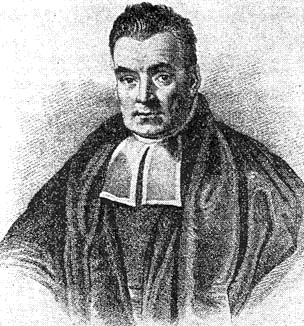
\includegraphics[scale=0.25]{images/thomas-bayes.png}
\caption*{{\bfseries Thomas Bayes} (1701 – 1761) \newline {\footnotesize Outlined for the first known time the solution to inverse probability.}}
\end{figure}
\end{minipage}\hspace{.05\textwidth}%
\begin{minipage}{0.45\textwidth}
\begin{figure}
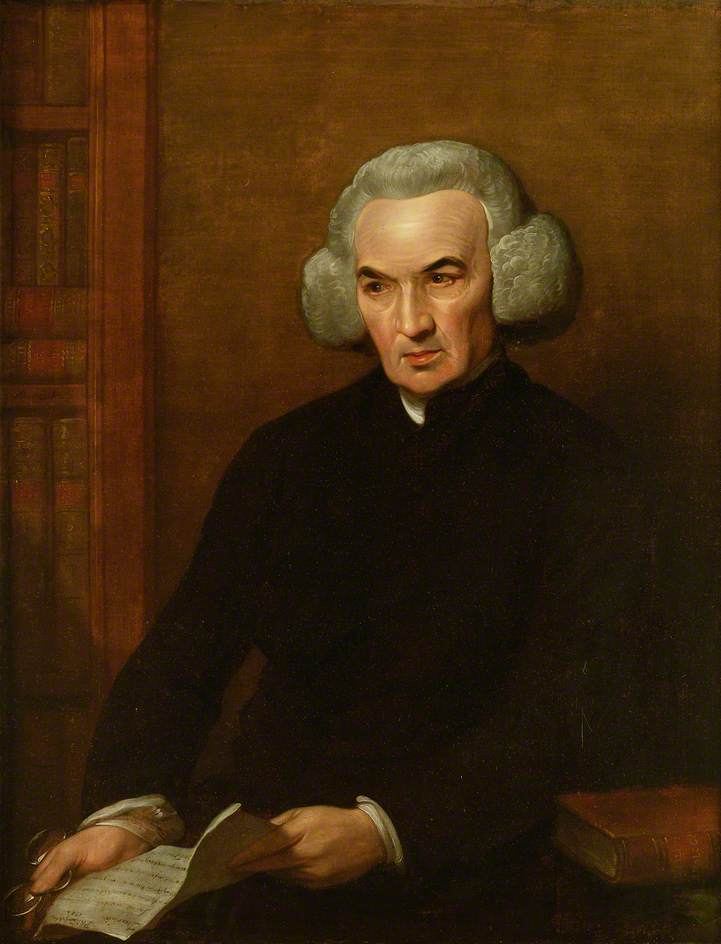
\includegraphics[scale=0.15]{images/richard-rrice-west.jpg}
\caption*{{\bfseries Richard Price} (1723 – 1791) \newline {\footnotesize Welsh Philosopher and Mathematician who published Bayes' notes.}}
\end{figure}
\end{minipage}
\end{center}

\end{frame}

\section{Bayesian Terminology}
\begin{frame}{}

{\large \textbf{Bayes' Theorem}}\vspace{1.5\baselineskip}\\

 Bayes' Theorem is $P(Y | X) = \frac{P(X | Y)\times P(Y)}{P(X)}$ where:
 
\vspace{1.5\baselineskip}

\begin{itemize}

\item $P(X)$ is evidence (data);

\vspace{1.5\baselineskip}

\item $P(Y)$ is prior probability (beliefs);

\vspace{1.5\baselineskip}

\item $P(X | Y)$ is the likelihood;

\vspace{1.5\baselineskip}

\item $P(Y | X)$ is the {\bfseries posterior probability}.

\end{itemize}

\end{frame}


%------------------------------------------%
% Takeaway
%------------------------------------------%
\section{Takeaway}
\begin{frame}{}

\begin{center}
\begin{minipage}{3.85in}

% Thank you.
\begin{center}

\includegraphics[width=.25in]{images/prayer.png} {\Large \textbf{Thank you for coming.}}\\
\end{center}

% Re-cap the lesson of the week.
\begin{center}
\begin{minipage}{\linewidth}
\begin{Block}{Lesson of the Day}

\vspace{\baselineskip}

\begin{itemize}

\item We can update our {\bfseries prior beliefs} as more and more {\bfseries data} comes to light using the {\bfseries likelihood} of observing the data.
\vspace{\baselineskip}

\end{itemize}

\end{Block}
\end{minipage}
\end{center}

\vfill

\end{minipage}
\end{center}

\end{frame}


%------------------------------------------%
% End
%------------------------------------------%
\end{document}
